% !TEX encoding = UTF-8 Unicode
\documentclass{beamer}
\usepackage{color}
\usepackage{url}
\usepackage[T2A]{fontenc}
\usepackage[utf8]{inputenc}
\usepackage{graphicx}
\usepackage{scrextend}
\usepackage[english,serbianc]{babel}
\usetheme{Copenhagen}
\usecolortheme{beaver}
\makeatother
\institute{\includegraphics[scale=0.175]{matf-logo.eps}}
\setbeamertemplate{footline}
{
  \leavevmode%
  \hbox{%
  \begin{beamercolorbox}[wd=1.0\paperwidth,ht=2.25ex,dp=1ex,center]{title in head/foot}%
    \usebeamerfont{title in head/foot}\insertshorttitle\hspace*{3em}
    \insertframenumber{} / \inserttotalframenumber\hspace*{1ex}
  \end{beamercolorbox}}%
  \vskip0pt%
}
\makeatletter
\setbeamertemplate{navigation symbols}{}

\date{\tiny{14. decembar 2019.}}

\title{\textbf{David Bader}}
\author{\small{Nikola Belaković, Vojkan Panić,\\Bogdan Damljanović, Filip Antonijević}}

\begin{document}
\frame{\titlepage}



% SLAJD 
\begin{frame}
\frametitle{Uvod}
\textbf{David Bader} (rođen 4. maja 1969.) ugledni je profesor i direktor Instituta za nauku o podacima na Tehnološkom institutu u Nju Džersiju. Ranije je bio profesor, predsedavajući Škole računarske nauke i inženjerstva i izvršni direktor računarstva visokih performansi na računarskom fakultetu u Džordžiji.  
\begin{center}
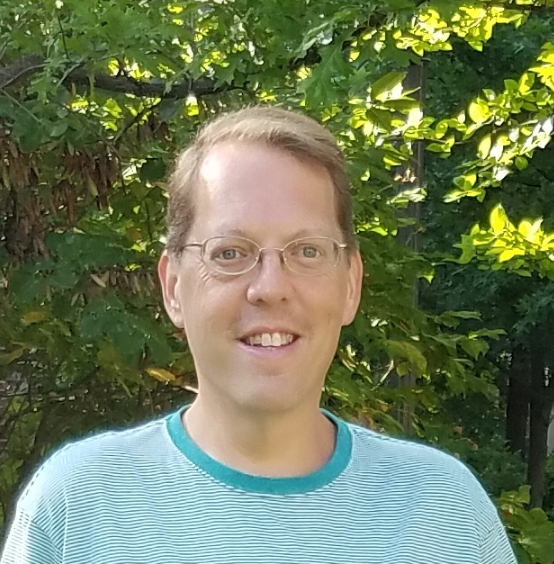
\includegraphics[scale=0.3]{David_Bader_2017.png}
\end{center}
\end{frame}


% SLAJD
\begin{frame}
\frametitle{Rani život}
\begin{itemize}
\item [-] Bader je sin profesora hemije Morisa Badera i njegove supruge Karen.
\item [-] Diplomirao je na Liberty High School u Betlehemu u Pensilvaniji.
\item [-] Postao je diplomirani inženjer iz oblasti računarskog inženjerstva i magistrirao na elektrotehnici na Univerzitetu Lihaj u Betlehemu.
\end{itemize}
\end{frame}

% SLAJD
\begin{frame}
\frametitle{Karijera}
Radio je na velikom broju položaja:
\begin{itemize}
\item     Profesor i regentski predavač na Univerzitetu u Novom Meksiku
\item     Profesor i prvi predsedavajući Škole računarske nauke i inženjerstva
\item 	  Profesor na Tehnološkom institutu u Nju Džersiju na katedri za računarske nauke
\item     Uređivač brojnih časopisa
\item     Vodeći istraživač na projektu Nvidia Echelon
\end{itemize}
\end{frame}

% SLAJD
\begin{frame}
\frametitle{Karijera}
\begin{itemize}

\item [-] Bader je suosnivao list Graph500 za vrednovanje računarskih platformi "Big Data".
\item [-] U aprilu 2019. godine najavljeno je da će Bader i njegov laboratorij u Georgia Techu sarađivati sa Envidiom da razviju rešenja za analizu podataka za svoje grafičke procesore.
\item [-] U julu 2019. Tehnološki institut u Nju Džersiju objavio je da će Bader obavljati funkciju direktora svog novoosnovanog Instituta za nauku o podacima na računarskom fakultetu Ying Wu.
\end{itemize}
\end{frame}




% SLAJD
\begin{frame}
\frametitle{Nagrade} 
Dobitnik je velikog broja nagrada:
\begin{itemize}
\item     NSF CAREER
\item     Alumni 2012
\item     Član AAAS-a i IEEE-a
\item     "Rock Star of High Performance Computing"
\item     Član "People to Watch"
\item 	  Golden Core član IEEE Computer Society
\item     Dekanova nagrada 2007. i izvanredna nagrada za istraživanje seniorskog fakulteta u 2014.
\end{itemize}

\end{frame}




% SLAJD
\begin{frame}
\frametitle{}
\begin{center}
Hvala na pažnji!
\end{center}
\begin{center}

\includegraphics[scale=0.5]{david.jpg}
\end{center}
\end{frame}


\end{document}
